%%%%%%%%%%%%%%%%%%%%%%%%%%%%%%%%%%%%%%%%%%%%%%%%%%%%%%%%%%%%%%%%%%%%%%%%
%    PulseAnalyse Manual										       %
%                                                                      				%
%    Latex Source Code                                                  %
%                                                                     				%
%    P.H. Charlton, adapted from IOP Latex Code           %
%%%%%%%%%%%%%%%%%%%%%%%%%%%%%%%%%%%%%%%%%%%%%%%%%%%%%%%%%%%%%%%%%%%%%%%%

%%%%% SETUP DOCUMENT %%%%%

\documentclass[12pt]{iopart}
\usepackage[pdftex]{graphicx}
\usepackage{color}
\usepackage{harvard}
\usepackage{multirow}
\usepackage{epstopdf}
\usepackage{adjustbox}
\usepackage{enumitem}
\hypersetup{hidelinks}
%\newcommand{\url}[1]{\textcolor{blue}{{\textit{#1}}}}
\usepackage{setspace}
\usepackage{scrextend}
\newcommand{\thresh}{\textit{k} }
\newcommand{\mean}[1]{\overline{#1}}
\newcommand{\pc}[1]{\textcolor{red}{{\textit{#1}}}}
\newcommand{\tb}[1]{\textcolor{blue}{{\textit{#1}}}}
\newcommand{\ja}[1]{\textcolor{red}{{\textit{#1}}}}
\newcommand{\eg}{\textit{e.g.} }
\newcommand{\ie}{\textit{i.e.} }
\newcommand{\pa}{\texttt{PulseAnalyse}}
\newcommand{\us}{\texttt{\_}}
\usepackage{cite}
\usepackage{array} % for tables
\newcolumntype{P}[1]{>{\centering\arraybackslash}p{#1}}
\usepackage{rotating}

\makeatletter
\def\bstctlcite{\@ifnextchar[{\@bstctlcite}{\@bstctlcite[@auxout]}}
\def\@bstctlcite[#1]#2{\@bsphack
	\@for\@citeb:=#2\do{%
		\edef\@citeb{\expandafter\@firstofone\@citeb}%
		\if@filesw\immediate\write\csname #1\endcsname{\string\citation{\@citeb}}\fi}%
	\@esphack}
\makeatother

% --------------- Making bibliography -------------- %

% see: http://anorien.csc.warwick.ac.uk/mirrors/CTAN/macros/latex/contrib/IEEEtran/bibtex/IEEEtran_bst_HOWTO.pdf

% and: http://tex.stackexchange.com/questions/164017/limiting-the-number-of-authors-in-the-references-with-ieeetran
\usepackage{filecontents} % To make the bib-file

\begin{filecontents}{refs.bib}
	@IEEEtranBSTCTL{IEEEexample:BSTcontrol,
		CTLuse_url = "no",
		CTLuse_forced_etal       = "yes",
		CTLmax_names_forced_etal = "3",
		CTLnames_show_etal       = "1", 
		CTLdash_repeated_names = "no" 
	}
	@article{paperOne,
		author = "Author First and Author Second and Author Third and Author Fourth",
		title = "Paper One Title",
		journal = "Awesome Journal",
		pages = "111--115",
		year = 2013
	}
	@incollection{paperTwo,
		author = "Author First and Author Second and Author Third",
		title = "Paper Two Title",
		booktitle = "Proc. of Collection",
		pages = "222--225",
		year = 2013
	}
\end{filecontents}



\begin{document}

\bstctlcite{IEEEexample:BSTcontrol}

%%%%% TITLE AND AUTHORS %%%%%

\title[P H Charlton \etal]{\pa{} \\ Extracting cardiovascular indices from pulse waves}

\author{Peter H. Charlton} % $^{1,2}$

\address{Department of Biomedical Engineering, King's College London, UK}

% \ead{peter.charlton@kcl.ac.uk}

%%%%% VERSION INFORMATION %%%%%

%\vspace{10pt}
%\begin{indented}
%\item[]Draft from \today
%\end{indented}

%%%%% ABSTRACT %%%%%

\begin{abstract}

This report presents \texttt{PulseAnalyse}, a Matlab \textregistered{} script for extracting cardiovascular indices from pulse waveforms.

\end{abstract}

%%%%% KEYWORDS %%%%%

% \noindent{\it Keywords}: respiratory modulation, biomedical signal processing, electrocardiography, photoplethysmography, respiratory rate

%%%%% SUBMISSION TO JOURNAL %%%%%
% \submitto{\PM}

%%%%% SPACING %%%%%
%\doublespacing

%%%%% INTRODUCTION %%%%%

\section{Summary}
\label{sec:intro}

Pulse waves contain a wealth of information on the cardiovascular (CV) system \cite{Elgendi2012,Gallagher}. Indices of CV state can be extracted from pulse waves by identifying fiducial points on the waves, and using these points to calculate indices. For example, CV indices can be extracted by identifying the systolic and diastolic peaks on the photoplethysmogram (PPG) wave, and measuring either the time delay between them or their relative amplitudes, as demonstrated in Figure \ref{fig:si_techniques}.
\begin{figure}[h]
	\centering
	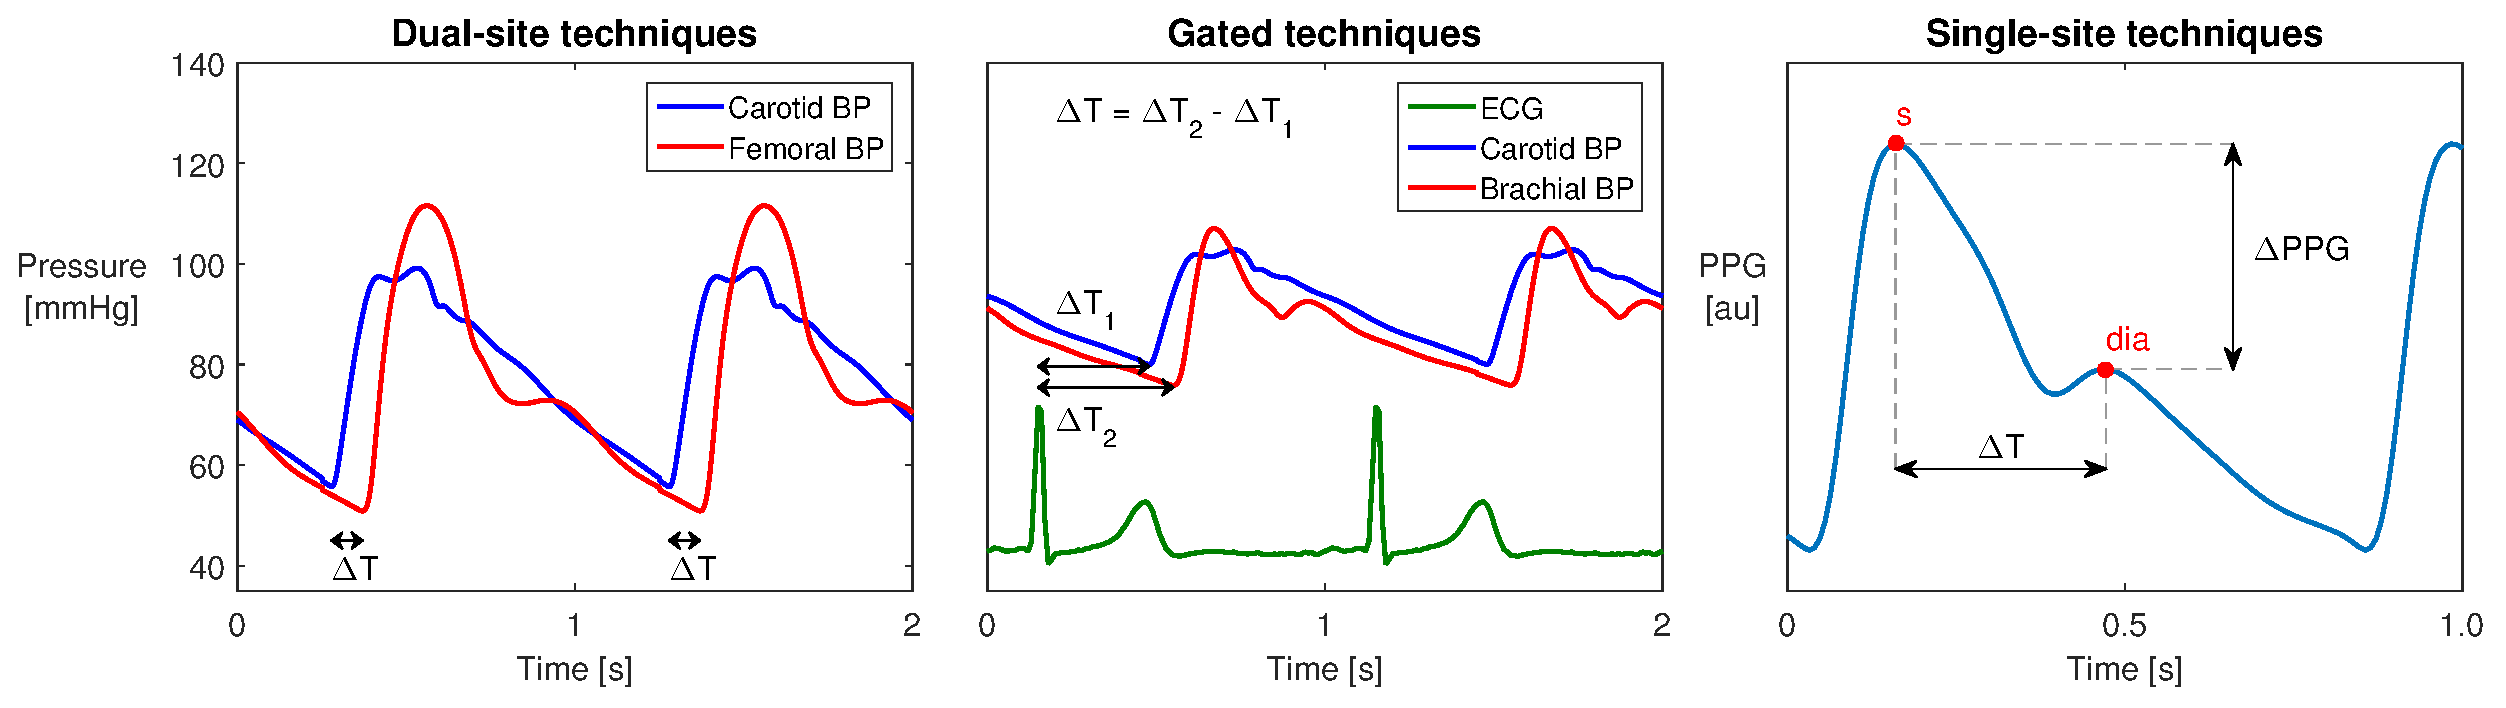
\includegraphics[width=0.4\linewidth, trim={28.1cm 0 0 0.8cm},clip]{./Figures/si_techniques_young.eps}
	%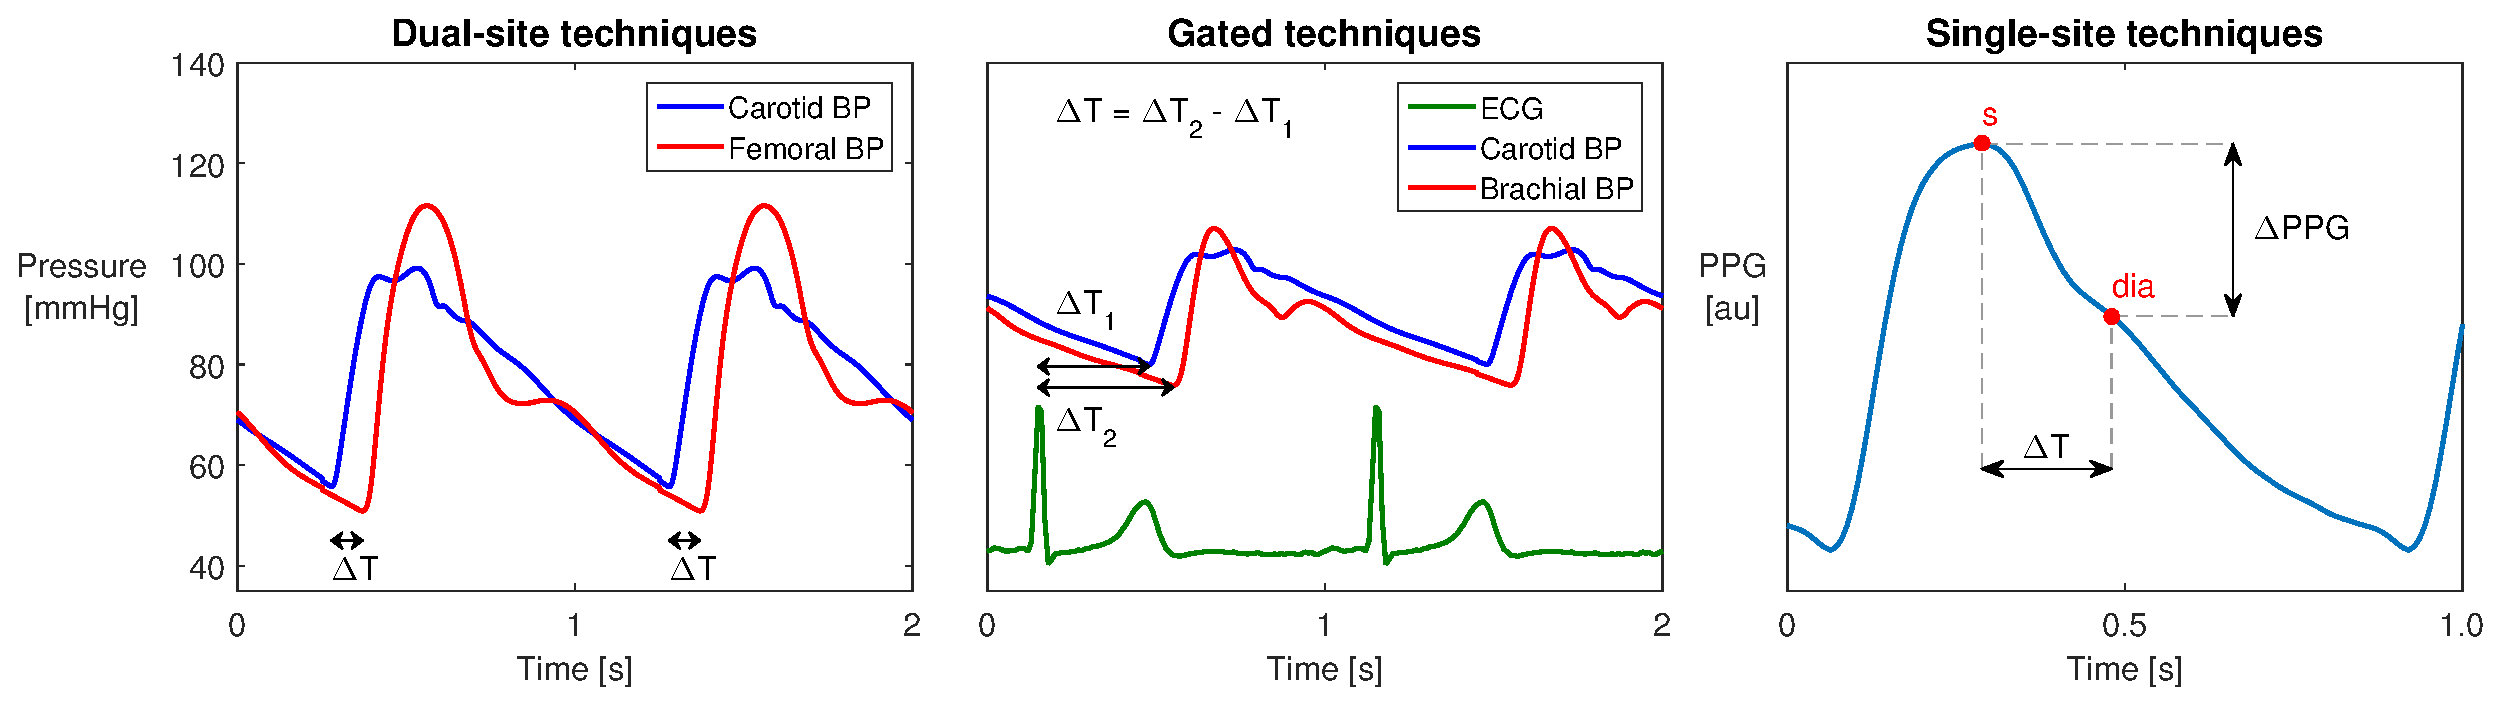
\includegraphics[width=0.4\linewidth, trim={28.1cm 0 0 0.8cm},clip]{./Figures/si_techniques_elderly.eps}
	\caption{Exemplary techniques for extracting CV indices from the PPG waveform. Two indices, $\Delta PPG$ and $\Delta T$, have been extracted by: (i) identifying the relevant fiducial points (the systolic and diastolic peaks in this case), and then measuring the difference in either the amplitude or time between these points.}
	\label{fig:si_techniques}
\end{figure}
A plethora of CV indices have been described in the literature. This report presents \pa, a Matlab \textregistered{} script for extracting many of these indices from pulse waves. \pa{} can be used to extract indices from either an individual pulse wave, or from a recording of a pulsatile signal (containing multiple pulse waves). It provides a standardised methodology for extracting indices, ensuring reproducibility.

\section{Calculating Cardiovascular Indices}

Several CV indices have been described in the literature. These are mostly extracted from pulse waves by: (i) identifying one or more fiducial points on either the pulse wave, or its first derivative, or its second derivative; and, (ii) extracting a measurement of the waveform morphology from the properties of these points.

A wide range of fiducial points have been used to calculate cardiovascular indices, as illustrated on exemplary PPG waveforms in Figure \ref{fig:fid_pts}.
\begin{figure}[t]
	\centering
	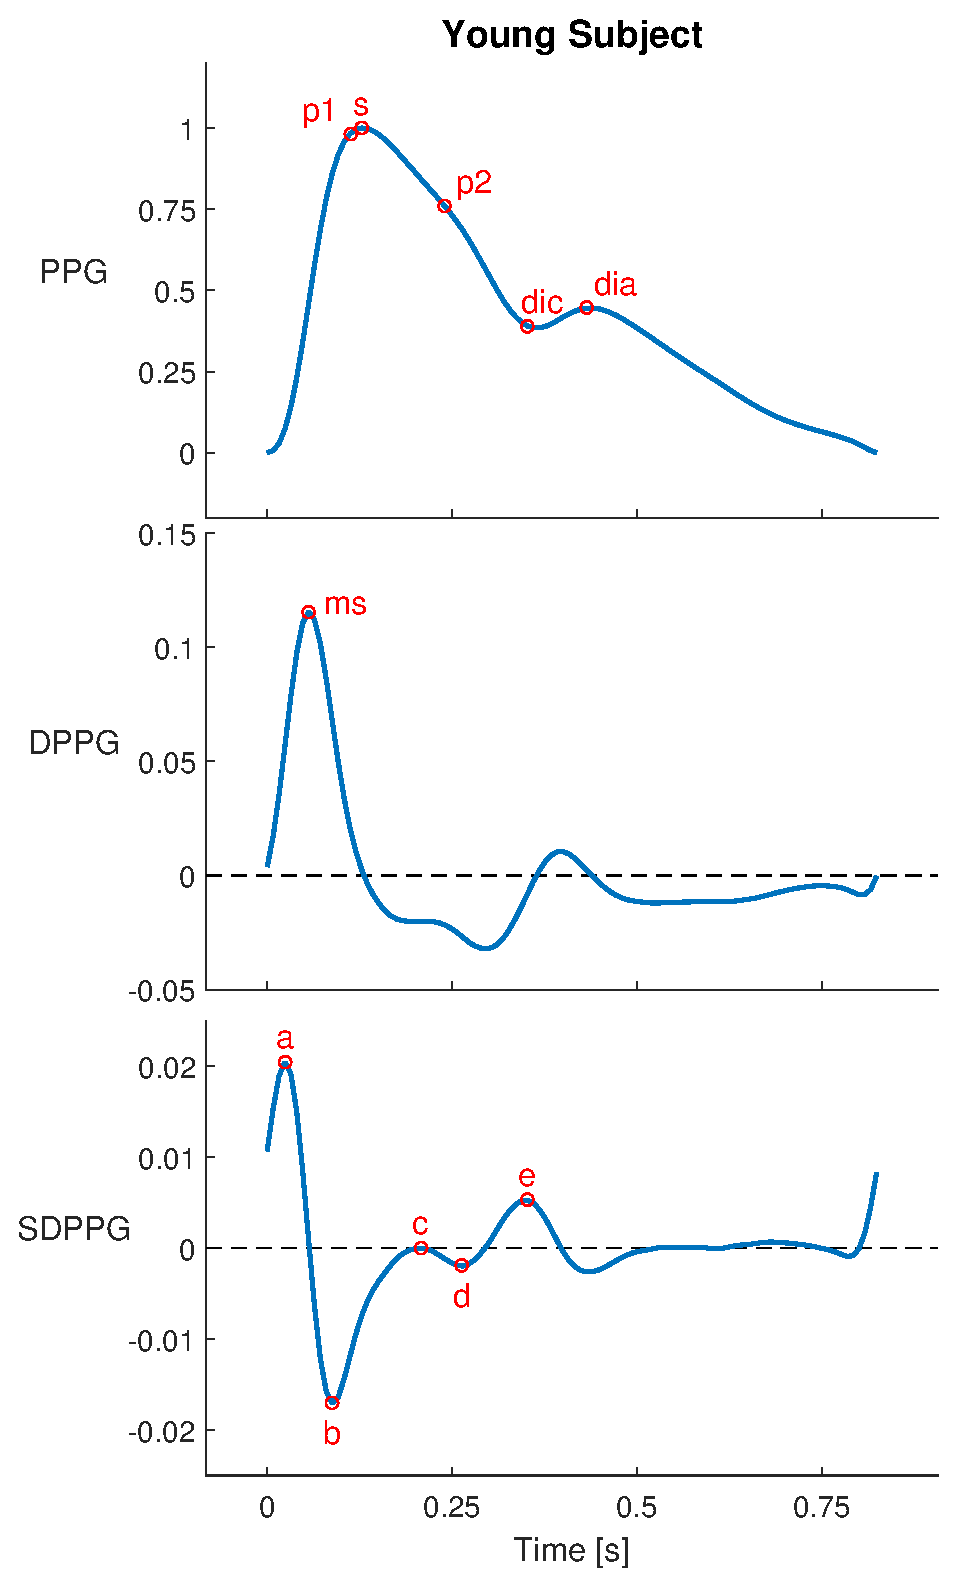
\includegraphics[width=0.49\linewidth]{./Figures/si_points_young.eps}
	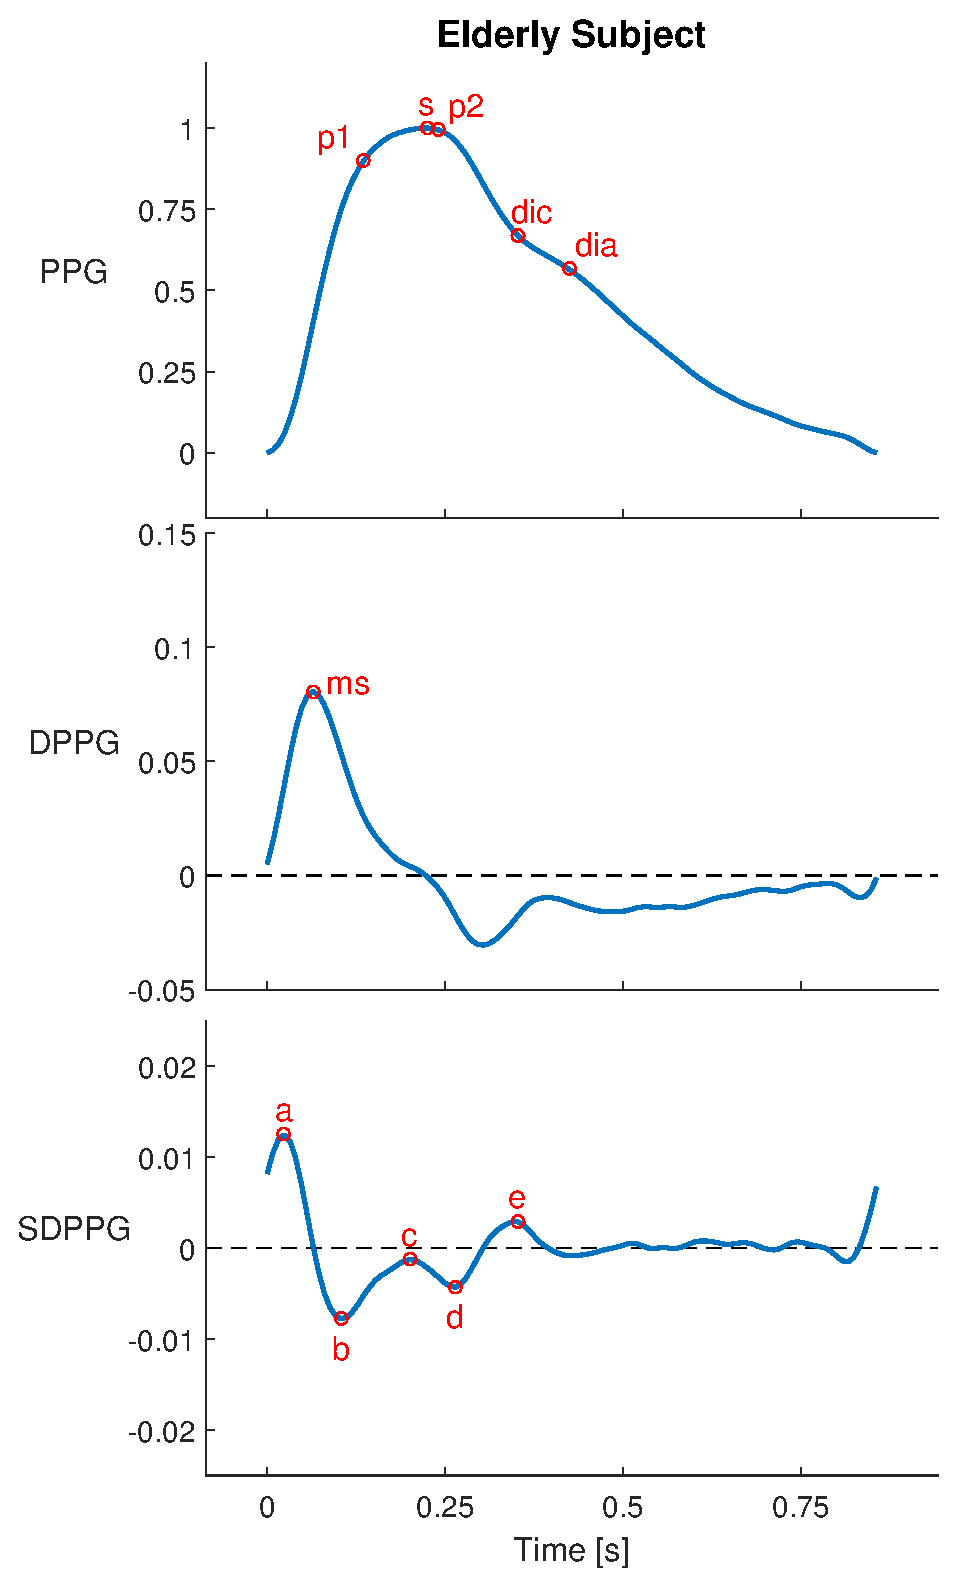
\includegraphics[width=0.49\linewidth]{./Figures/si_points_elderly.eps}
	\caption{The fiducial points which have been used to calculate CV indices, illustrated on the PPG waveform (upper row), its first derivative (DPPG, middle row), and second derivative (SDPPG, lower row). The following points on the  waveform (upper row) have been used: $p1$, the early systolic component; $p2$, the late systolic component; $s$, the systolic peak; $dic$, the dicrotic notch; and $dia$, the diastolic peak. The point of maximum slope, $ms$, has been identified using the first derivative. The following points have been identified using the second derivative \cite{Elgendi2012}: $A$, the early systolic positive wave; $B$, the early systolic negative wave; $C$, the late systolic reincreasing wave; $D$, the late systolic redecreasing wave; and $E$, the early diastolic increasing wave (corresponding to the dicrotic notch).}
	\label{fig:fid_pts}
	% Generated using ppg_fiducial_points2.m
\end{figure}
There is no consensus on the optimal methodology for identifying these fiducial points on pulsatile waveforms.

Once fiducial points have been identified, a CV index can be calculated as a function of the co-oridinates of those points (in time and amplitude). Table \ref{tab:SIs_res} summarises the CV indices which are calculated by \pa.

\begin{table}[t]
	\caption{\label{tab:SIs_res} CV indices calculated from a pulse wave (PW), its first (DPW) and second derivatives (SDPW), by \pa. Definitions: $h$ - subject height; $T$ - duration of cardiac cycle.}
	\vspace{0.5cm}
	\centering
	\renewcommand{\arraystretch}{1.2}
	\footnotesize
	\begin{tabular}{p{2cm}p{2cm}cp{8.3cm}c}
		\hline
		\textbf{Signal} & \textbf{Approach} & \textbf{Abbr.} & \textbf{Formula} & \textbf{Ref} \\
		\hline
		\multirow{12}{*}{\textbf{PW}} & Timings & $\Delta T$ & $t(dia) - t(s)$ & \cite{Chowienczyk1999} \\
		& & $SI$ & $h / (t(dia) - t(s))$ & \cite{Millasseau2002} \\
		& & $CT$ & $t(s)$ & \cite{Alty2003} \\
		& & $CT/h$& $t(s)/h \:$ & \cite{Wu2010} \\
		& & $prop_s$ & $t(s)/T$ & \cite{Wu2010} \\
		& & $t_{sys}$ & $t(dic)$ & \cite{Ahn2017} \\
		& & $t_{dia}$ & $T - t(dic)$ & \cite{Ahn2017} \\
		& & $t_{ratio}$ & $t(s) / t(dic)$ & \cite{Ahn2017} \\
		& & $prop_{\Delta T}$ & $(t(dia) - t(s)) / T$ & \cite{Ahn2017} \\
		& & $t_{p1-dia}$ & $t(dia) - t(p1)$ & \cite{Peltokangas2017a} \\
		& & $t_{p2-dia}$ & $ t(dia) - t(p2)$ & \cite{Peltokangas2017a} \\
		& Amplitudes & $AI$ & $(PW(p2) - PW(p1)) / PW(s)$ & \cite{Takazawa1998} \\ 
		& & $RI$ & $PW(dia) / PW(s)$ & \cite{Chowienczyk1999} \\
		& & $RI_{p1}$ & $PW(dia) / PW(p1)$ & \cite{Peltokangas2017a} \\
		& & $RI_{p2}$ & $PW(dia) / PW(p2)$ & \cite{Peltokangas2017a} \\
		& & $ratio_{p2-p1}$ & $PW(p2)  / PW(p1)$ & \cite{Peltokangas2017a} \\
		& Areas & $A1$ & area from pulse foot to dicrotic notch & \cite{Ahn2017} \\
		& & $A2$ & area from dicrotic notch to pulse end & \cite{Ahn2017} \\
		& & $IPA$ & $A2/ A1$ & \cite{Ahn2017} \\
		\hline
		\multirow{1}{*}{\textbf{DPW}} & Amplitudes & $ms$ & $DPW(ms) / PW(s) $ & \cite{Alty2003} \\  
		\hline
		\multirow{6}{*}{\textbf{SDPW}} & Amplitudes & $b/a$ & $SDPW(b)/SDPW(a)$ & \cite{Takazawa1998} \\
		& & $c/a$ & $SDPW(c)/SDPW(a)$ & \cite{Takazawa1998} \\
		& & $d/a$ & $SDPW(d)/SDPW(a)$ & \cite{Takazawa1998} \\
		& & $e/a$ & $SDPW(e)/SDPW(a)$ & \cite{Takazawa1998} \\
		& & $AGI$ & $(SDPW(b)-SDPW(c)-SDPW(d)-SDPW(e))/SDPW(a)$ & \cite{Takazawa1998} \\
		& & $AGI_{inf}$ & $(SDPW(b)-SDPW(e))/SDPW(a)$ & \cite{Hyun2008} \\
		& & $AGI_{mod}$ & $(SDPW(b)-SDPW(c)-SDPW(d))/SDPW(a)$ & \cite{Ushiroyama2005} \\
		& Timings & $t_{b-c}$ & $t(c) - t(b)$ & \cite{Ahn2017} \\
		& & $t_{b-d}$ & $t(d) - t(b)$ & \cite{Ahn2017} \\
		& Slopes & $slope_{b-c}$ & $d / dt$ of straight line between $b$ and $c$, normalised by $a$ & \cite{Ahn2017} \\
		& & $slope_{b-d}$ & $d / dt$ of straight line between $b$ and $d$, normalised by $a$ & \cite{Ahn2017} \\
		\hline
		\multirow{2}{*}{\textbf{Combined}} & multiple & $IPAD$ & $(A2/ A1) + d/a$ & \cite{Ahn2017} \\
		& Amplitudes & $k$ & $SDPW(s) / ( (PW(s)-PW(ms)) / PW(s) ) $& \cite{Wei2013} \\
		\hline
	\end{tabular}
\end{table}



\section{Using \pa}

\pa{} can be used to calculate CV indices from either a pulsatile signal containing several pulses, or a single pulse wave. The input data, $S$, should be prepared as a structure with two fields: $S.v$, a vector of signal amplitudes, and $S.fs$, the sampling frequency of the signal. At its simplest, \pa can be called using
\begin{center}
	\texttt{cv\us inds = PulseAnalyse(S);}
\end{center}
where \texttt{cv\us inds} is a structure containing individual fields for each of the calculated CV indices (named according to the abbreviations listed in Table \ref{tab:SIs_res}). Each index's field is itself a structure, containing the calculated value (\eg{} \texttt{cv\us inds.SI.v}, which is a median in the case of multiple pulses), and raw values for each pulse (\texttt{cv\us inds.SI.raw}) if the input signal contains multiple pulses.

Additional functionality can be exploited by specifying additional inputs. Firstly, if the subject's height is provided in $S.ht$ then those CV indices which require height will be calculated. Secondly, options can be specified as a second input using
\begin{center}
	\texttt{cv\us inds = PulseAnalyse(S, options);}
\end{center}
where \texttt{options} is a structure containing the following logical fields:
\begin{itemize}
	\item \texttt{exclude\us low\us quality\us data}: whether or not to exclude pulses with a low signal quality in the calculation of a median value for each CV index (only applicable when using an input signal with multiple pulses).
	\item \texttt{do\us plot}: whether or not to plot an example pulse with fiducial points annotated (similar to those in Figure \ref{fig:fid_pts}).
\end{itemize}

Additional outputs can also be obtained using
\begin{center}
	\texttt{[cv\us inds, fid\us pts, pulses, S\us filt] = PulseAnalyse(S);}
\end{center}
where \texttt{fid\us pts} is a structure containing the indices of each fiducial point; \texttt{pulses} is a structure containing the indices of the onsets and peaks of each pulse, and the signal quality of each pulse (a logical where 1 indicates high signal quality); and \texttt{S\us filt} is the filtered pulsatile signal to which these indices correspond.

\section{Methods}

\pa consists of three stages: (i) pre-processing a pulsatile signal; (ii) detecting fiducial points on each pulse of the signal; and (iii) calculating CV indices from these points. The methods used at each stage are now described in turn.

\subsection{Pre-processing}

Firstly, pre-processing steps are performed to facilitate extraction of CV indices from a pulsatile signal (consisting of multiple pulse waves). Firstly, the signal is filtered to remove irrelevant low (\textless{} 0.067 Hz) and high frequency (\textgreater{} 35 Hz) content, which can impact the values of CV indices. Secondly, individual pulse waves are identified within the signal using the segmentation algorithm described in \cite{Karlen2012}. A third, optional step consists of identifying pulses with a low signal quality. This is performed using the algorithm described in \cite{Orphanidou2015}.

The filtered pulse waves were differentiated three times to calculate the first, second and third derivatives. Derivatives were calculated using Savitsky-Golay filtering with the following transfer function:
\begin{equation}
H(z) = \frac{0.2 + 0.1 z^{-1} - 0.1 z^{-3} - 0.2 z^{-4}}{1}
\end{equation}
The time-shifted derivatives were then time-aligned with the original signal. 

\subsection{Detecting Fiducial Points}

\pa{} identifies fiducial points on the pulse wave (PW) as follows. Firstly, the following points are identified on the second derivative (SDPW):
\begin{itemize}
	\item \textbf{\emph{a}}: The point of maximum value on the SDPW prior to the last local minimum on the SDPW.
	\item \textbf{\emph{b}}: The first local minimum on the SDPW following \emph{a}.
	\item \textbf{\emph{e}}: The maximum of the SDPW between \emph{b} and the pulse end.
	\item \textbf{\emph{d}}: The last local minimum on the SDPW before \emph{e}.
	\item \textbf{\emph{c}}: The maximum of the SDPW between \emph{b} and \emph{d}.
	\item \textbf{\emph{f}}: The first local minimum of the SDPW after \emph{e}.
\end{itemize}
The following points on the PW are then identified:
\begin{itemize}
	\item \textbf{\emph{s}}: The maximum of the PPG.
	\item \textbf{\emph{dic}}: Coincident with \emph{e}.
	\item \textbf{\emph{dia}}: Coincident with \emph{f}.
\end{itemize}
The maximum of the first derivative (DPW), denoted \emph{ms}, is then identified. Finally, the following points are detected using the third derivative (TDPW):
\begin{itemize}
	\item \textbf{\emph{p1}}: The first local maximum of TDPW following \emph{ms}.
	\item \textbf{\emph{p2}}: The first local minimum of TDPW following \emph{c}.
\end{itemize}

\subsection{Calculating CV Indices}

CV indices are calculated from the time and amplitude co-ordinates of the fiducial points using the formulae in Table \ref{tab:SIs_res}.

\section{Further Work}
\label{sec:prev_work}

Other approaches have also been used to extract CV indices from pulse waves, which could also be implemented in \pa{}. Several techniques have been proposed which involve decomposing the pulse waveform into its component parts prior to assessment of arterial stiffness, including: (i) eigen decomposition, from which eigenvalues can be calculated which are indicative of arterial stiffness \cite{Angarita-jaimes2006}; (ii) decomposition into Gaussians from which indices of arterial stiffness can be calculated \cite{Rubins2008}; and (iii) decomposition into lognormal functions from which indices can be calculated \cite{Huotari2011}. Furthermore, some techniques require additional information beyond that of the pulse shape, such as: (i) the level of the PPG's DC offset (used in \cite{Sawada2001} to calculate the normalised pulse volume); (ii) simultaneous blood pressure measurement (used in \cite{Tanaka2011} to calculate a finger elasticity index); and (iii) simultaneous measurement of pulse waves at multiple anatomical sites (such as the finger and toe \cite{Tsai2005,Peltokangas2017} and right and left toes \cite{Allen2008,Allen2005}). Other techniques are not yet suitable for automated analysis, such as the use of a 10-element windkessel model in \cite{Zahedi2007} to predict the pulse shape, in which the manually optimised windkessel parameters were proposed as indices of arterial stiffness.

\newpage


\section*{References}


\bibliographystyle{IEEEtran}
\bibliography{refs,refs2,refs_extra}

\end{document}

